\documentclass[10pt,letterpaper]{article}
\usepackage[T1]{fontenc}
\usepackage{lmodern}
\usepackage[margin=1.16in,top=1.02in,bottom=1.02in]{geometry}
\usepackage{amsmath,amssymb,amsthm}
\usepackage{array,booktabs,tabularx}
\usepackage{tikz}
\usetikzlibrary{arrows.meta}
\usepackage[font=small,labelfont=bf]{caption}
\usepackage{float}
\usepackage[colorlinks=true,linkcolor=bandblue,citecolor=bandblue,urlcolor=bandblue]{hyperref}
\definecolor{graphink}{HTML}{24344A}
\definecolor{bandblue}{HTML}{16678A}
\definecolor{gaprust}{HTML}{9C4517}
\hypersetup{
  pdftitle={Polynomial Kernelization for Maximum Shortest-Cycle Coverage on Planar Graphs},
  pdfauthor={Haorui Yu, Dingkai Hu}
}
\newtheorem{theorem}{Theorem}
\newtheorem{lemma}{Lemma}
\newtheorem{corollary}{Corollary}
\newcommand{\forest}{\mathcal F}
\newcommand{\tree}{\mathcal T}
\newcommand{\cactus}{\mathcal C}
\newcommand{\figurecredit}{TikZ schematic drafted from the construction with OpenAI Codex (GPT-6-based) assistance.}
\newcommand{\artifact}{\href{https://github.com/scmypapa/Polynomial-Kernelization-for-Maximum-Shortest-Cycle-Coverage-on-Planar-Graphs/tree/reproducibility-v2}{archived GitHub snapshot}}
\raggedbottom
\setlength{\emergencystretch}{1.5em}
\title{Polynomial Kernelization for Maximum Shortest-Cycle\\ Coverage on Planar Graphs}
\author{Haorui Yu\textsuperscript{a}, Dingkai Hu\textsuperscript{b}\\[0.55em]
  {\small\itshape\textsuperscript{a}Sichuan University, Chengdu, China}\\[-0.12em]
  {\small\itshape\textsuperscript{b}Tongji University, Shanghai, China}}
\date{}

\begin{document}
\maketitle
\begin{abstract}
Given a simple undirected planar graph with positive integer edge weights, a positive integer \(k\), and a nonnegative threshold \(T\), the \emph{Planar Maximum Shortest-Cycle Coverage} problem asks whether \(k\) distinct globally shortest simple cycles have an edge union of weight at least \(T\). Agrawal et al.\ asked whether the problem admits a polynomial kernel parameterized by \(k\). We give a deterministic polynomial-time kernel with total encoding length \(O(k^{300})\) bits, including the binary edge weights and threshold. In the planar dual, a minimum-cut cactus yields \(O(k)\) paths of ordinary cuts and \(O(k^2)\) exceptional cuts. The embedding organizes the ordinary cuts through monotone bands and nested same-side intervals. Two finite propagation stages and one-sided overlap charges allow a polynomial-size family of locally optimal selections to retain a global optimum. We compress the union of their primal cycles and then apply Frank--Tardos weight compression.
\end{abstract}

\section{Introduction and main theorem}
Let \(G=(V,E)\) be a finite simple undirected planar graph with a binary-encoded weight function \(w:E\to\mathbb Z_{>0}\). We write \(w(F)=\sum_{e\in F}w(e)\) for \(F\subseteq E\). The weighted girth \(\lambda\) of \(G\) is the minimum weight of a simple cycle. A globally shortest simple cycle has weight \(\lambda\), and we distinguish cycles by their edge sets.

\smallskip
\noindent\textbf{Problem (Planar Maximum Shortest-Cycle Coverage).}
Given \(G,w\), an integer \(k\ge 1\), and a nonnegative integer \(T\), decide whether there are \(k\) distinct globally shortest simple cycles \(C_1,\ldots,C_k\) with
\[
w\!\left(\bigcup_{i=1}^k E(C_i)\right)\ge T.
\]
The instance is a no-instance when \(G\) is acyclic. We parameterize by \(k\).

Positive weights imply that at threshold \(T=k\lambda\) the selected cycles must be pairwise edge-disjoint. Bentert et al.\ gave a polynomial kernel for this special case \cite{Bentert2025}. Agrawal et al.\ obtained a single-exponential parameterized algorithm for the planar diverse coverage problem and identified kernelization for coverage without a diversity constraint as an open problem \cite[Section~6]{Agrawal2026}.

\begin{theorem}\label{thm:main}
Planar Maximum Shortest-Cycle Coverage has a deterministic polynomial kernel parameterized by \(k\). The output is an equivalent simple planar instance with total encoding length \(O(k^{300})\) bits, including its binary edge weights and threshold.
\end{theorem}

The proof passes to minimum cuts in the planar dual. The cactus gives paths on which a cut is represented by a position. A band can couple choices across entire paths, and the graph of these path-level dependencies can have degree greater than two. We propagate a polynomial number of boundaries through the bands and across endpoint gaps. For a fixed optimum this yields blocks whose two-variable interactions form paths and cycles. The same-side overlap between blocks admits a one-sided bound that is tight at the optimum. Local dynamic programs can then replace each interaction component independently. Finally, the marked cuts yield a small graph and permit weight compression.

\section{Planar duality, minimum-cut cactus, and the ordinary-cut forest}
\subsection{Dual equivalence and preliminary tests}
Test acyclicity first. If \(G\) has more than one component, connect the components by unit-weight bridges and take a plane embedding of the connected graph. The bridges belong to no simple cycle. In the dual \(D\), delete the loops corresponding to primal bridges. Positive capacities imply that both shores of every global minimum cut induce connected subgraphs. Otherwise the shore components would yield cuts of total capacity at least twice the dual minimum value. Therefore each global minimum cut is a bond. Plane cycle--bond duality identifies the global minimum cuts of \(D\) with the globally shortest simple cycles of \(G\), preserving edge identities, capacity \(\lambda\), and union weights.

Let \(n=|V(D)|\) and \(q\) be the number of global minimum cuts. The weighted minimum-cut bound gives \(q\le\binom n2\) \cite{KargerStein}. Compute \(\lambda\) and enumerate the cuts as in Section~\ref{sec:construction}. If \(q<k\) or \(T>k\lambda\), output a unit-weight triangle with \((k',T')=(2,0)\), the same fixed no-instance as for an acyclic input. Henceforth \(k\le q\le\binom n2\). This bound makes fixed powers of \(k\) polynomial in the input length even when \(k\) is binary encoded.

For an edge \(uv\) in \(D\), the minimum \(u\)-\(v\) cut has capacity \(\lambda\) exactly when \(uv\) belongs to a global minimum cut. Contract all edges belonging to no global minimum cut. Delete every loop created by contraction and retain parallel edges with their identities. Each contracted edge has both ends on the same shore of every global minimum cut. Thus every such cut survives, together with its edges and the capacity of any union. Every cut in the contracted graph lifts to a cut of \(D\), so the contraction preserves the minimum-cut family. Write \(H\) for the resulting connected loopless plane multigraph.

\subsection{Exact cactus representation and the pure-bridge forest}
Take an exact minimum-cut cactus \((\cactus,\phi)\) of \(H\) \cite{FleinerFrank,HeHuangSaranurak}. Replace each two-edge cycle by one bridge. The basic cuts are the deletion of a bridge and the deletion of two distinct edges of one remaining cycle. The shores of all global minimum cuts of \(H\), including singleton shores, are exactly the preimages of the basic-cut shores. Replace each cactus cycle of length at least three by a hub adjacent to its vertices to obtain the block tree \(\tree\). For a cactus vertex \(v\), let \(B_v=\phi^{-1}(v)\) be its bag and let \(q(v)=\deg_{\tree}(v)\).

\begin{lemma}\label{lem:bag}
Each bag \(B_v\) spans no edge of \(H\) and satisfies \(|B_v|\le q(v)\). The instance is a yes-instance whenever \(H\) has at least \(6k\) vertices of weighted degree \(\lambda\).
\end{lemma}
\begin{proof}
Vertices in one bag lie on the same shore of every global minimum cut. All edges of \(H\) belong to such a cut, so the bag is independent. The components of \(\tree-v\) pull back to sets \(S_1,\ldots,S_{q(v)}\) partitioning \(V(H)\setminus B_v\). Each \(S_i\) is a shore of a global minimum cut: the incident tree edge comes either from a cactus bridge or from a cycle whose two edges at \(v\) can be deleted. Hence
\[
 |B_v|\lambda
 \le\sum_{u\in B_v}\deg_w(u)
 =w(\delta B_v)
 \le\sum_{i=1}^{q(v)}w(\delta S_i)=q(v)\lambda .
\]
In particular each leaf bag is a singleton of degree \(\lambda\). Among \(6k\) vertices of weighted degree \(\lambda\), a six-coloring of their underlying simple planar graph gives an independent set of at least \(k\) vertices. Their singleton cuts are edge-disjoint and have union capacity \(k\lambda\). The algorithm can output the unit-weight triangle with \((k',T')=(1,3)\).
\end{proof}

We may now assume that \(\tree\) has \(\ell<6k\) leaves. A cactus bag is \emph{pure-bridge} if its tree degree is two and both incident edges are cactus bridges. Suppress any empty pure-bridge bag, since its two bridges represent the same cut.

\begin{lemma}\label{lem:forest}
Every remaining pure-bridge bag is a singleton \(\{x\}\) with \(\deg_w(x)>\lambda\). If two pure-bridge bags are adjacent, their vertices \(x,y\) are joined by an edge of \(H\) that is crossed only by the cut of their common bridge.
\end{lemma}
\begin{proof}
By Lemma~\ref{lem:bag}, a nonempty pure-bridge bag has at most two vertices. In the two-vertex case both have degree \(\lambda\), and their singleton cuts split the bag, a contradiction. If a singleton pure-bridge bag had degree \(\lambda\), its singleton cut would have to separate it from both nonempty branches of \(\tree-v\). Each branch contains a nonempty leaf bag. A basic cut cannot simultaneously cut the two incident bridges, so such a singleton cut is impossible.

For the two branches \(A,B\) at \(x\), set \(a=w(x,A)\), \(b=w(x,B)\), and \(c=w(A,B)\), using the weight of edges between the indicated sets. The two incident bridge cuts give \(a+c=b+c=\lambda\), hence \(a=b=\deg_w(x)/2>\lambda/2\). For adjacent pure-bridge vertices \(x,y\), the edges incident to \(x\) in the intervening cut have capacity greater than \(\lambda/2\), and so do those incident to \(y\). They intersect in an actual \(xy\) edge. A basic cut separates these adjacent bags only when it deletes their common bridge.
\end{proof}

Choose one such private edge for every pair of adjacent pure-bridge bags. Together with vertices incident to none of these edges as isolated vertices, they form a path forest \(\forest\). Call the cuts of these forest edges \emph{ordinary}, and all other global minimum cuts \emph{exceptional}.

\begin{corollary}\label{cor:forest}
The forest \(\forest\) has \(p=O(k)\) components and there are \(O(k^2)\) exceptional cuts after deduplication. An edge \(uv\) of \(H\) crosses precisely the ordinary cuts on the path in \(\tree\) from \(\phi(u)\) to \(\phi(v)\). Each exceptional cut puts each component of \(\forest\) on a single shore.
\end{corollary}
\begin{proof}
The tree satisfies \(\sum_{\deg(v)\ge 3}\deg(v)\le 3\ell-6\). Each cycle hub has degree equal to the length of its cycle, so \(\sum_K |K|=O(k)\) over all long cactus cycles \(K\). Leaves, branching bags, and the bags incident to these hubs have total tree degree \(O(k)\) and contain \(O(k)\) vertices by Lemma~\ref{lem:bag}. Deleting those bags and the hubs leaves \(O(k)\) chains of pure-bridge bags. This bounds \(p\). There are \(O(k)\) bridges incident to a non-pure bag and \(\sum_K\binom{|K|}{2}\le(\sum_K |K|)^2/2=O(k^2)\) basic long-cycle cuts. The last statements follow from the bridge path in \(\tree\) and the fact that every forest edge is private to its ordinary cut.
\end{proof}

\subsection{Deterministic polynomial-time construction}\label{sec:construction}
For a fixed root vertex, the minimum over minimum cuts separating it from each other vertex gives \(\lambda\). To enumerate the global minimum cuts without duplicating complements, fix the root outside the listed shore and branch on membership of the other vertices. For a prefix with both assigned shores nonempty, contract each assigned shore and test whether the two resulting terminals have minimum cut value \(\lambda\). If the inside shore is still empty, try each unassigned vertex as an inside representative. Expand exactly the feasible prefixes. Each lies on one of at most \(q\) root-to-leaf paths of length \(n\), and every visited infeasible prefix is a child of a feasible one. Thus the enumeration uses \(O(n(q+1))\) prefix tests and \(O(n^2(q+1))=O(n^4)\) flow computations.

Apply the capacitated construction of Fleiner and Frank \cite[Lemma~2, Theorem~7, Remark~1]{FleinerFrank} to \(H\). A two-vertex graph gives a bridge. When all minimum cuts have a singleton shore and the graph has at least three vertices, a star has one leaf per singleton cut, with the other vertices in the center bag. A \emph{proper} cut here means a cut whose shores each have size at least two. If proper cuts exist and each proper minimum cut has a crossing partner, the capacitated form of their Lemma~2 says that the graph, after aggregating each parallel bundle, is a cycle with bundle capacities \(\lambda/2\). Use that cycle with singleton bags. In the remaining case choose an uncrossed proper minimum cut. Contract its two shores in separate subproblems, keep the minimum value \(\lambda\), and glue the two returned cacti at the nodes carrying the two contracted vertices as in their construction. The uncrossed cut ensures that every original minimum cut is represented in one of the two subproblems.

The cut list in each subproblem determines the case by testing all pairs for crossing. For a split with shore sizes \(a,b\ge2\), child sizes are \(a+1,b+1\) and their size-minus-two measures add to \(a+b-2\). Each nonroot subproblem has measure at least one, so there are \(O(n)\) calls. Each uses the enumeration bound above and polynomial-time tests on the shores. Contracted capacities are sums of input capacities, so their bit lengths and all flow computations are polynomial in the binary input size.

\section{Band decomposition along the two sides of the planar forest}
For a forest path \(P_r=(v_0,\ldots,v_\ell)\), take a thin disk neighborhood whose boundary, from head to tail, has sides \(0\) and \(1\). Use a coordinate line for \(P_r\) and put \(v_j\) at \(j\). Let \(N=|V(H)|+|E(H)|+2\), counting parallel edges individually. At \(v_j\), enumerate the \(d_j\) incident half-edges outside \(\forest\) in the order along each side, interleaving the two side orders arbitrarily. For \(a=1,\ldots,d_j\), give the \(a\)-th event coordinate
\[
             j+\frac{a}{8N}.
\]
All these coordinates are distinct and lie in \((j,j+1/4)\). Each isolated vertex has \(j=0\) and a split of its cyclic order into two side intervals. Use \(-1,\ell+1\) as the end coordinates of the line. The ordinary cut of \(v_jv_{j+1}\) will receive a coordinate in \((j+1/4,j+3/4)\), so the event--cut order agrees with the vertex order.

Contract each forest path and split the resulting vertex at the two ends of the disk. The two side vertices \((r,0),(r,1)\) are joined by one auxiliary edge. The resulting connected plane multigraph \(\widetilde H\) has \(2p\) vertices and \(p\) auxiliary edges. Cutting the rotation at each auxiliary half-edge recovers the linear rotation order on that side (Figure~\ref{fig:split}).

\begin{figure}[H]
\centering
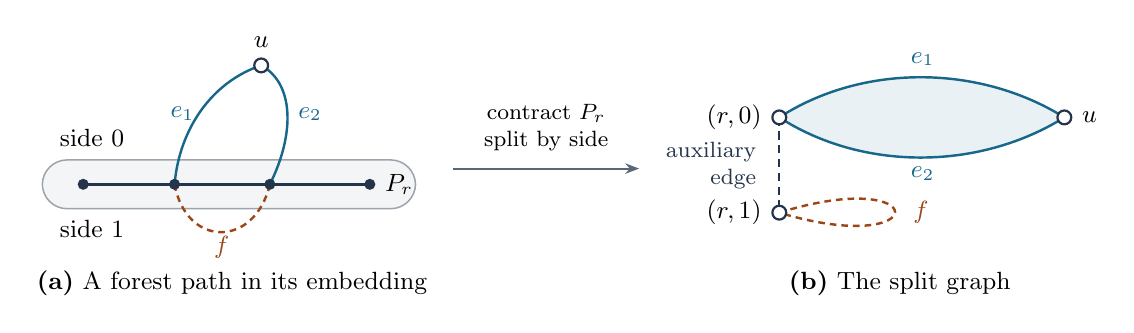
\begin{tikzpicture}[
  x=1cm,y=1cm,font=\small,
  vertex/.style={inner sep=0pt,circle,fill=graphink,minimum size=4pt},
  portvertex/.style={inner sep=0pt,circle,draw=graphink,fill=white,line width=.8pt,minimum size=5pt},
  forest/.style={draw=graphink,line width=1.2pt,line cap=round},
  essential/.style={draw=bandblue,line width=.88pt,line cap=round},
  inessential/.style={draw=gaprust,line width=.88pt,dash pattern=on 2.4pt off 1.8pt},
  aux/.style={draw=graphink,line width=.75pt,densely dashed}]
  \path[draw=graphink!45,fill=graphink!5,line width=.55pt,rounded corners=9pt]
    (0.16,0.94) rectangle (4.90,1.56);
  \coordinate (v0) at (.68,1.25);
  \coordinate (v1) at (1.84,1.25);
  \coordinate (v2) at (3.05,1.25);
  \coordinate (v3) at (4.32,1.25);
  \coordinate (u) at (2.94,2.76);
  \draw[forest] (v0)--(v1)--(v2)--(v3);
  \draw[essential] (v1) .. controls (1.90,1.95) and (2.31,2.55) .. (u);
  \draw[essential] (v2) .. controls (3.37,1.89) and (3.36,2.53) .. (u);
  \draw[inessential] (v1) .. controls (1.99,.44) and (2.86,.44) .. (v2);
  \foreach \v in {v0,v1,v2,v3} {\node[vertex] at (\v) {};}
  \node[portvertex,label={above:$u$}] at (u) {};
  \node[bandblue] at (1.94,2.15) {$e_1$};
  \node[bandblue] at (3.56,2.14) {$e_2$};
  \node[gaprust] at (2.44,.45) {$f$};
  \node[anchor=west] at (.26,1.84) {side 0};
  \node[anchor=west] at (.26,.68) {side 1};
  \node[anchor=west] at (4.39,1.25) {$P_r$};

  \draw[graphink!75,line width=.75pt,-{Stealth[length=5pt]}] (5.38,1.45)--(7.74,1.45);
  \node[align=center,font=\footnotesize] at (6.56,1.97) {contract \(P_r\)\\split by side};

  \coordinate (r0) at (9.52,2.10);
  \coordinate (r1) at (9.52,.89);
  \coordinate (w) at (13.14,2.10);
  \path[fill=bandblue!9]
    (r0) .. controls (10.57,2.78) and (12.05,2.78) .. (w)
    .. controls (12.05,1.42) and (10.57,1.42) .. (r0) -- cycle;
  \draw[essential] (r0) .. controls (10.57,2.78) and (12.05,2.78) .. (w);
  \draw[essential] (r0) .. controls (10.57,1.42) and (12.05,1.42) .. (w);
  \draw[aux] (r0)--(r1);
  \draw[inessential] (r1) .. controls (11.48,1.50) and (11.48,.30) .. (r1);
  \node[portvertex,label={left:$(r,0)$}] at (r0) {};
  \node[portvertex,label={left:$(r,1)$}] at (r1) {};
  \node[portvertex,label={right:$u$}] at (w) {};
  \node[bandblue,anchor=south] at (11.34,2.63) {$e_1$};
  \node[bandblue,anchor=north] at (11.34,1.60) {$e_2$};
  \node[graphink,anchor=east,align=right,font=\footnotesize] at (9.35,1.49) {auxiliary\\edge};
  \node[gaprust,anchor=west] at (11.10,.89) {$f$};
  \node at (2.57,-.01) {\textbf{(a)}~A forest path in its embedding};
  \node at (11.05,-.01) {\textbf{(b)}~The split graph};
\end{tikzpicture}

\caption{Path contraction and splitting. The disk about \(P_r\) records the two side orders. After splitting, \(e_1,e_2\) bound a two-edge face and form one band. The dashed loop \(f\) cuts off a disk containing no other vertex. \figurecredit}
\label{fig:split}
\end{figure}

\subsection{Same-side edges and nested intervals}
A \emph{same-side edge} is an edge outside \(\forest\) that becomes a loop at a side vertex in \(\widetilde H\) and cuts off a disk containing no other vertex. The sector inside that disk excludes the auxiliary half-edge, since the auxiliary edge joins a different vertex. In the linear side order, each half-edge between the two loop events belongs to a loop in the same disk. These inner loops also enclose vertex-free disks. Thus the open event interval of a same-side edge contains no event of an edge remaining after all same-side edges have been deleted. Planarity forbids alternating endpoints for two same-side edges in the same side order, so their intervals are disjoint or nested.

For such an edge \(e\), write \((l_e,r_e)\) for the open interval between its two event coordinates. Corollary~\ref{cor:forest} shows that \(e\) belongs to an ordinary cut at \(x\) on its path exactly for \(l_e<x<r_e\), and no other cut covers it. Each forest edge, in turn, belongs only to its own ordinary cut.

\subsection{Monotone bands}
Delete the same-side edges from \(\widetilde H\). Form a multigraph of edge adjacencies whose vertices are the remaining non-auxiliary edges. Each face bounded by two distinct such edges contributes one adjacency between them.

\begin{lemma}\label{lem:bands}
Each component of the edge-adjacency graph is a path, called a \emph{band}. Its two sets of half-edges are contiguous in their linear side orders, and corresponding endpoints match monotonically. There are at most \(7p-6\) bands except in the single-auxiliary-edge case, which has zero bands.
\end{lemma}
\begin{proof}
Each edge has at most two incident faces, so the adjacency graph has maximum degree two. In a cyclic component both face sides of each edge would be used. Consequently the predecessor and successor of every one of its half-edges in the rotation at that vertex would also belong to the component. Following the rotation would reach the auxiliary half-edge, which has no such adjacency. This also rules out a cycle formed by two adjacencies between the same pair.

Along a path of adjacencies, each two-edge face pairs the two edges' half-edges at its two corners. At an internal edge of the path, the predecessor and successor faces use opposite sides of each half-edge. Thus the two endpoint sequences advance in fixed directions along their respective linear orders. They are disjoint blocks of half-edges even when their side vertex is the same.

After deleting the same-side edges the plane graph has no one-edge face. A loop bounding such a face would cut off a vertex-free disk and would already have been deleted. In each band, remove edges from an end until one edge remains. Each removal merges a two-edge face with the other face of that edge and preserves the latter's boundary length. Connectivity is preserved. If the other face was another two-edge face using only non-auxiliary edges, its two edges already belonged to the same band. Thus each surviving two-edge face has an auxiliary incidence. In the single-edge case the claim is immediate. Otherwise, writing \(E,V,F\) for the edge, vertex, and face counts of the resulting graph and \(f_2\) for its number of two-edge faces, we have \(f_2\le 2p\) and \(2E\ge 3F-f_2\). Euler's formula with \(V=2p\) yields \(E\le 8p-6\). Subtracting the \(p\) auxiliary edges gives the claimed bound.
\end{proof}

For each endpoint block of a band \(B\), take the closed interval from its first event minus \(1/(32N)\) to its last event plus \(1/(32N)\). Call the two intervals its \emph{ports}. The event spacing makes distinct ports on the same side disjoint and each port nondegenerate, including for a one-edge band. By Lemma~\ref{lem:bands}, matching the corresponding events and the appropriate port ends gives a strictly monotone piecewise-linear bijection \(f_B\) between the ports. A point on a coordinate line lies in at most one port per side.

On each side, reserve the events of the remaining non-auxiliary edges and the two end coordinates as separators. The open intervals between consecutive separators are the \emph{gaps} of that side. Both events of a same-side edge lie in one gap, by the vertex-free disk property.

\section{Two finite partitions and stable levels}
\subsection{Propagation along band maps}
Let \(M_0\) consist of the ends of the path lines and of the ports. Given \(M_j\), add to it all images of its points under any applicable \(f_B\) or \(f_B^{-1}\) to obtain \(M_{j+1}\). All coordinates are labeled by their path line.

\begin{lemma}\label{lem:bandmarks}
We have \(|M_j|=O(p(j+1))\). The image of an open interval contained in a port and disjoint from \(M_{j+1}\) is disjoint from \(M_j\).
\end{lemma}
\begin{proof}
Consider the graph of point-to-point band transports, with edges viewed in both directions. Each line point has at most two neighbors because there is at most one port per side. Starting from \(|M_0|=O(p)\) seeds, a shortest walk extends from each seed in at most two directions, with at most one continuation per direction at successive vertices. This bounds the vertices reached by depth \(j\). A point of \(M_j\) in the image of the given interval would have its preimage in \(M_{j+1}\), which proves the second claim.
\end{proof}

Set \(d=k+2\) and \(L=(6k^2+1)d\). Precompute \(M_{L+1}\). The initial events, port ends, and path ends have \(O(\log N)\)-bit numerators and denominators. Each affine piece of a band map or its inverse has coefficients of \(b=O(\log N)\) bits, since interpolation uses a constant number of arithmetic operations on initial coordinates. For example, for \(\alpha=a_1/a_2\), \(\beta=b_1/b_2\), and \(x=u/v\), a step \(x\mapsto\alpha x+\beta\) gives
\[
              \frac{a_1 b_2 u+a_2 b_1 v}{a_2 b_2 v}.
\]
The maximum of the numerator and denominator bit lengths increases by at most \(O(b)\), and reducing the fraction can only decrease it. All marks therefore have \(O((L+1)\log N)\) bits. Here \(L=O(k^3)=O(n^6)\), with \(n\) the number of dual vertices before contraction. This gives polynomial bit time for choosing affine pieces, propagating points, and sorting them. The dependence on \(N\) accounts for arbitrarily many parallel edges even when \(n\) is small.

Choose each ordinary cut coordinate from \(|M_{L+1}|+1\) equally spaced interior points of its prescribed interval. At least one avoids \(M_{L+1}\). Its image under any applicable band map avoids \(M_L\), since the inverse image of a mark of \(M_L\) belongs to \(M_{L+1}\). The equally spaced points and the later test points chosen as interval midpoints have polynomial bit length.

Fix a witnessing optimum \(S^\star\) of \(k\) cuts. As \(j\) increases, monitor these monotone separation events.
\begin{enumerate}
\item A point of \(M_j\) lies strictly between two distinct selected ordinary cuts on one coordinate line.
\item Two distinct selected ordinary cuts lie in opposite ports of the same band and a point of \(M_j\) lies strictly between the image of the first and the second. Monitor both directions.
\end{enumerate}
The number of events is at most \(\binom{k}{2}+2k(k-1)\le 6k^2\), since a cut uses at most one port per side. Each event first becomes true at most once. Among \(t\in\{0,d,\ldots,6k^2d\}\), some window from \(M_t\) to \(M_{t+d}\) has no change in any event. Enumerate all these choices of \(t\).

Call the open cells of \(M_t\) \emph{original intervals}, and those of \(M_{t+1}\) \emph{fine intervals}. At a stable level \(t\), all selected cuts in an occupied original interval \(R\) lie in one fine interval \(I_R\) and remain unseparated through \(M_{t+d}\). Because \(M_t\) contains the port ends, an original interval on a given side is either inside one port or disjoint from all port interiors. Lemma~\ref{lem:bandmarks} puts the image of \(I_R\) under a containing port in a single original interval. An event located exactly at an \(M_t\) mark is assigned a degenerate original interval consisting of that point. Such intervals contain no possible cut.

\subsection{Propagation across gaps}
For fixed \(t\), set \(E_0=M_t\). A gap is \emph{hit at level \(i\)} when its interior contains a point of \(E_i\). Adjoin the endpoints of all gaps hit at level \(i\) on either side to obtain \(E_{i+1}\) (Figure~\ref{fig:propagation}).

\begin{figure}[H]
\centering
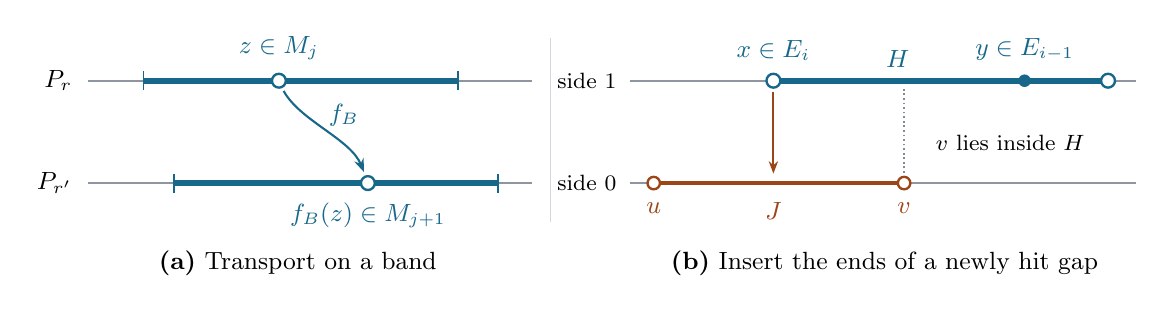
\begin{tikzpicture}[
  x=1cm,y=1cm,font=\small,
  track/.style={draw=graphink!52,line width=.6pt},
  band/.style={draw=bandblue,line width=2.1pt,line cap=butt},
  gap/.style={draw=gaprust,line width=1.45pt,line cap=butt},
  marker/.style={circle,draw=bandblue,line width=.85pt,fill=white,inner sep=0pt,minimum size=5pt},
  endpt/.style={circle,draw=gaprust,line width=.85pt,fill=white,inner sep=0pt,minimum size=4.5pt}]
  \draw[track] (.82,2.34)--(6.45,2.34);
  \draw[track] (.82,1.04)--(6.45,1.04);
  \draw[band] (1.52,2.34)--(5.51,2.34);
  \draw[band] (1.91,1.04)--(6.02,1.04);
  \foreach \u in {1.52,5.51} {\draw[bandblue,line width=.7pt] (\u,2.22)--(\u,2.46);}
  \foreach \u in {1.91,6.02} {\draw[bandblue,line width=.7pt] (\u,.92)--(\u,1.16);}
  \draw[bandblue,line width=.75pt,-{Stealth[length=4.8pt]}]
    (3.30,2.21) .. controls (3.51,1.83) and (4.15,1.60) .. (4.32,1.18)
    node[midway,above right,inner sep=1pt] {$f_B$};
  \node[marker] at (3.24,2.34) {};
  \node[marker] at (4.37,1.04) {};
  \node[anchor=east] at (.74,2.34) {$P_r$};
  \node[anchor=east] at (.74,1.04) {$P_{r'}$};
  \node[bandblue,above] at (3.24,2.48) {$z\in M_j$};
  \node[bandblue,below] at (4.37,.91) {$f_B(z)\in M_{j+1}$};

  \draw[graphink!20,line width=.55pt] (6.69,.54)--(6.69,2.88);
  \draw[track] (7.7,2.34)--(14.13,2.34);
  \draw[track] (7.7,1.04)--(14.13,1.04);
  \node[anchor=east,font=\footnotesize] at (7.65,2.34) {side 1};
  \node[anchor=east,font=\footnotesize] at (7.65,1.04) {side 0};
  \draw[band] (9.52,2.34)--(13.77,2.34);
  \node[marker] at (9.52,2.34) {};
  \node[marker] at (13.77,2.34) {};
  \node[circle,fill=bandblue,inner sep=1.6pt] at (12.71,2.34) {};
  \node[bandblue,above] at (11.10,2.39) {$H$};
  \node[bandblue,above] at (9.52,2.47) {$x\in E_i$};
  \node[bandblue,above] at (12.71,2.47) {$y\in E_{i-1}$};
  \draw[gap] (8.00,1.04)--(11.18,1.04);
  \node[endpt] at (8.00,1.04) {};
  \node[endpt] at (11.18,1.04) {};
  \draw[gaprust,line width=.69pt,-{Stealth[length=4.5pt]}] (9.52,2.20)--(9.52,1.16);
  \draw[graphink!57,densely dotted,line width=.65pt] (11.18,1.17)--(11.18,2.23);
  \node[gaprust,below] at (8.00,.92) {$u$};
  \node[gaprust,below] at (9.52,.92) {$J$};
  \node[gaprust,below] at (11.18,.92) {$v$};
  \node[anchor=west,font=\footnotesize] at (11.46,1.55) {$v$ lies inside $H$};
  \node at (3.48,.02) {\textbf{(a)}~Transport on a band};
  \node at (10.93,.02) {\textbf{(b)}~Insert the ends of a newly hit gap};
\end{tikzpicture}

\caption{The two propagation rules. (a) A band transports the mark \(z\) to the opposite port. (b) The new mark \(x\) is an endpoint of the already hit gap \(H\) and now hits \(J=(u,v)\) on the opposite side. The inward endpoint \(v\) lies inside \(H\), so \(v\) generates no new hit at the next level. \figurecredit}
\label{fig:propagation}
\end{figure}

\begin{lemma}\label{lem:gapmarks}
For all \(i\ge 0\), \(|E_i|\le(1+8i)|M_t|\). Removing the closures of the gaps hit at level \(i\), on both sides, leaves at most one open interval in each original interval. Ordinary cut coordinates avoid \(E_i\).
\end{lemma}
\begin{proof}
Let \(\mathcal A_i\) be the gaps first hit at level \(i\). Each \(E_0\) point hits at most one gap per side, so \(|\mathcal A_0|\le 2|E_0|\). For \(J\in\mathcal A_i\) with \(i\ge 1\), a witnessing point \(x\in J\cap(E_i\setminus E_{i-1})\) was inserted as the endpoint of a gap \(H\in\mathcal A_{i-1}\) on the other side. Take \(y\in H\cap E_{i-1}\). Since \(J\) contains \(x\) and excludes \(y\), an endpoint \(v\) of \(J\) lies on the segment from \(x\) to \(y\), after \(x\) and possibly at \(y\). Hence \(v\) lies strictly inside \(H\). At \(v\) the side of \(J\) has no gap interior, and the other side has only the already hit gap \(H\). This endpoint cannot generate a fresh hit. The argument applies to every gap in \(\mathcal A_i\) for \(i\ge1\), so each has at most one endpoint that can generate a first hit at the next level. Each endpoint can hit at most one gap on the opposite side. It follows that \(|\mathcal A_1|\le 2|\mathcal A_0|\) and \(|\mathcal A_{i+1}|\le|\mathcal A_i|\) for \(i\ge 1\). Summing the two new endpoints per first hit gives the bound on \(|E_i|\).

Each hit gap's closure contains a seed in \(M_t\) or touches the closure of an earlier hit gap whose endpoint hit it. Thus every connected component of the union of the closures meets \(M_t\). In an original interval these components can intrude only from its two ends, leaving at most one open interval. The new marks are event or path end coordinates and hence are distinct from ordinary cut coordinates. The seed marks were avoided by construction.
\end{proof}

For \(S^\star\) monitor, on both sides of every selected ordinary cut, whether the cut lies in a hit gap. These at most \(2k\) flags change monotonically. There is some \(s\in\{0,\ldots,2k\}\) with no flag change from \(E_s\) to \(E_{s+1}\), and the algorithm enumerates all such \(s\).

The open cells of \(E_{s+1}\) are the \emph{subintervals}. A subinterval is \emph{closed} on a side if it lies in a gap hit at level \(s\) on that side, and \emph{open} on that side otherwise. The endpoints of those hit gaps are in \(E_{s+1}\), so the side status is constant within each subinterval. The candidate domain is the set of ordinary cuts in its intersection with \(I_R\) that avoid every gap hit at level \(s+1\) on each of its open sides. Stability retains every selected cut. On a closed side all comparisons with band endpoints on that side are fixed. All points of \(E_{s+1}\setminus M_t\) lie in the closures of gaps hit at level \(s+1\). By Lemma~\ref{lem:gapmarks}, the complement of these closures in \(R\) is one interval or empty and contains no point of \(E_{s+1}\). Thus at most one subinterval in \(R\) is open on both sides and has a nonempty candidate domain.

\section{Local objectives and one-sided charging}
Fix \(S^\star\), its stable \((t,s)\), its exceptional cuts, and its occupied original intervals. All selected cuts in \(R\) stay in \(I_R\). Say \(R\) is \emph{self-paired} if \(I_R\) lies in the two opposite ports of one band and its images from both ports are contained in \(R\). Such an \(R\) is a single block with domain \(I_R\). In each other occupied \(R\), each subinterval containing a selected cut is a block with the guarded candidate domain of Section~4.2. Every block must remain nonempty. Their order implies that the blocks supplying the first and last cuts of each original interval remain fixed. Domains of distinct blocks are disjoint.

\subsection{The exact same-side overlap}
The weight of covered forest edges is the sum of the private forest-edge weights of the selected ordinary cuts. For the same-side edges on a fixed side of a path, add their covered weight separately for each block. If an interval is covered by two blocks, it is covered by every intervening nonempty block. Subtracting the duplicate weight for each adjacent pair therefore counts every covered edge once.

Consider adjacent active blocks \(U<V\) on the same path line, and let \(x=\max S_U\) and \(y=\min S_V\). There is a known mark \(m\in E_{s+1}\) separating the two domains, using an \(M_t\) boundary when the blocks are in different original intervals. In particular \(x<m<y\). On the side in question, let \(\mathcal N_m\) be the same-side edges whose intervals strictly contain \(m\). Define
\[
 A_m(x)=\sum_{\substack{e\in\mathcal N_m\\l_e<x<r_e}}w(e),
 \qquad
 B_m(y)=\sum_{\substack{e\in\mathcal N_m\\l_e<y<r_e}}w(e).
\]

\begin{lemma}\label{lem:overlap}
The weight covered by both \(U\) and \(V\) on the given side is
\begin{equation}
     \operatorname{overlap}(S_U,S_V)=\min\{A_m(x),B_m(y)\}.
     \label{eq:overlap}
\end{equation}
Fix the side attaining the minimum at \(S^\star\). Its prefix weight is an upper bound on the overlap for every permitted simultaneous replacement and is tight at \(S^\star\). If a non-self-paired block is open on a side, its overlap with another block on that side is identically zero.
\end{lemma}
\begin{proof}
An interval hit in both blocks contains \(x,m,y\). The intervals containing \(m\) form an inclusion chain. Those covering \(x\) and those covering \(y\) are prefixes of this chain in decreasing order of inclusion. Their intersection is the shorter prefix, whose weight is the smaller of the two prefix weights. Figure~\ref{fig:overlap} shows an example. Fixing either prefix as the charge upper-bounds the minimum for every replacement, and fixing an attaining prefix gives equality at \(S^\star\).

An interval covering an open block and another block would lie in a gap containing the separating mark \(m\). This gap is hit at level \(s+1\), and the candidate domain on the open side excludes it.
\end{proof}

\begin{figure}[H]
\centering
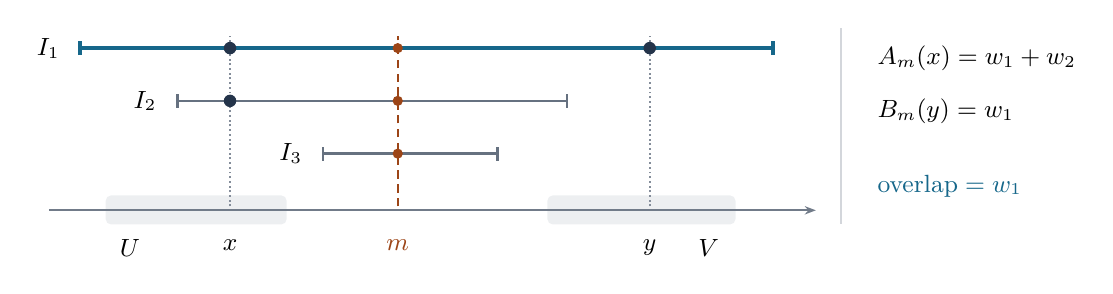
\begin{tikzpicture}[
  x=1cm,y=1cm,font=\small,
  track/.style={draw=graphink!65,line width=.65pt},
  allinterval/.style={draw=graphink!70,line width=.95pt},
  winner/.style={draw=bandblue,line width=1.45pt},
  included/.style={circle,fill=graphink,inner sep=0pt,minimum size=4.5pt}]
  \path[fill=graphink!8,rounded corners=2pt] (1.47,.64) rectangle (3.77,1.01);
  \path[fill=graphink!8,rounded corners=2pt] (7.08,.64) rectangle (9.47,1.01);
  \draw[track,-{Stealth[length=4pt]}] (.75,.82)--(10.49,.82);
  \node[below=2pt] at (1.78,.64) {$U$};
  \node[below=2pt] at (9.13,.64) {$V$};
  \draw[graphink!56,densely dotted,line width=.7pt] (3.05,.87)--(3.05,3.04);
  \draw[gaprust,densely dashed,line width=.75pt] (5.18,.87)--(5.18,3.04);
  \draw[graphink!56,densely dotted,line width=.7pt] (8.38,.87)--(8.38,3.04);
  \node[below=2pt] at (3.05,.64) {$x$};
  \node[gaprust,below=2pt] at (5.18,.64) {$m$};
  \node[below=2pt] at (8.38,.64) {$y$};

  \foreach \l/\r/\h/\k/\sty in {1.15/9.94/2.88/1/winner,
                               2.38/7.33/2.21/2/allinterval,
                               4.23/6.45/1.54/3/allinterval} {
    \draw[\sty] (\l,\h)--(\r,\h);
    \draw[\sty] (\l,\h-.09)--(\l,\h+.09) (\r,\h-.09)--(\r,\h+.09);
    \node[anchor=east] at (\l-.14,\h) {$I_{\k}$};
  }
  \foreach \a in {(3.05,2.88),(8.38,2.88),(3.05,2.21)}
    {\node[included] at \a {};}
  \node[gaprust,circle,fill=gaprust,inner sep=1.3pt] at (5.18,2.88) {};
  \node[gaprust,circle,fill=gaprust,inner sep=1.3pt] at (5.18,2.21) {};
  \node[gaprust,circle,fill=gaprust,inner sep=1.3pt] at (5.18,1.54) {};

  \draw[graphink!20,line width=.55pt] (10.81,.65)--(10.81,3.13);
  \node[anchor=west] at (11.15,2.75) {$A_m(x)=w_1+w_2$};
  \node[anchor=west] at (11.15,2.08) {$B_m(y)=w_1$};
  \node[bandblue,anchor=west] at (11.15,1.13) {$\mathrm{overlap}=w_1$};
\end{tikzpicture}

\caption{Nested intervals and the overlap charge. All \(I_j\) contain \(m\), and \(w_j\) is the weight of \(I_j\). The left extremum \(x\) hits \(I_1,I_2\), and the right extremum \(y\) hits \(I_1\). Fixing the right charge at this witness gives \(B_m(y')\) for any replacement, which bounds its actual overlap from above. \figurecredit}
\label{fig:overlap}
\end{figure}

\subsection{Band groups and the interaction graph}\label{sec:bandgroups}
For a band \(B\), group its edges by the ordered pair \((R,R')\) of original intervals containing their endpoints, with the order given by the two ports. We call the resulting group \((B,R,R')\). A degenerate interval at a mark is allowed as an endpoint.

\paragraph{Coverage from outside the endpoint intervals.}
An exceptional cut keeps each forest component on one shore, so it covers either every edge of the group or none. For an ordinary cut in a third original interval, the relative shore of each endpoint is fixed over that endpoint's entire interval. On its own forest path this follows from the order of the cut and event coordinates. Off that path it follows from Corollary~\ref{cor:forest}, since any route in \(\tree\) leaving a pure-bridge path exits at one end. Hence such a cut also covers the whole group or none. Whole-group coverage by these cuts depends only on the fixed exceptional cuts and occupied original intervals. It gives a constant contribution.

\paragraph{Groups with \(R=R'\).}
For a self-paired \(R\), the two port images of \(I_R\) stay in \(R\), so all varying band edges at \(R\) are internal. Their support is the interval \((l_e,r_e)\) on the same forest path by Corollary~\ref{cor:forest}. Only ordinary cuts of \(R\) can cover these edges. Put their intervals into the in-block objective. If \(R\) is non-self-paired and a port image of \(I_R\) lies in \(R\), it is disjoint from \(I_R\). An intersection would put \(I_R\) in both ports of this band and force both images into \(R\) by Lemma~\ref{lem:bandmarks}. Thus all edges varying through that port have their opposite endpoints on a fixed side of \(I_R\), and one extremal cut controls their coverage.

\paragraph{Groups with \(R\ne R'\).}
When the group is free of whole-group coverage, its path direction at each endpoint interval is fixed by \(\tree\). On one forest path this is the order of the two intervals. Between different forest paths it is the end of each path through which the route exits. A cut nearer that end covers a superset of the group edges covered by a cut farther from the end. Thus the block supplying the extreme toward the other interval controls coverage, using its minimum cut coordinate toward the left and its maximum toward the right. For a given interval side only one group can vary: a varying edge must have its event in \(I_R\), and the port map sends all of \(I_R\) into one original interval.

Place a two-variable edge between the two supplying blocks for a group precisely in the following case. Both endpoint intervals are occupied and non-self-paired, the images are mutual
\[
                f_B(I_R)\subseteq R',\qquad f_B^{-1}(I_{R'})\subseteq R,
\]
and both supplying blocks are open on their participating sides. The score of this edge is the weight of the group edges covered by either supplying extremum.

Table~\ref{tab:outside} gives the other cases. When mutuality fails, at most one end has varying coverage. Indeed, if both fine intervals contained group events, even from different edges, Lemma~\ref{lem:bandmarks} would force mutuality. From the varying side all relevant opposite events lie in the image of its fine interval, entirely on one side of the opposite fine interval. They therefore share a fixed opposite coverage bit. If an image \(f_B(I_R)\subset R'\) points into a self-paired \(R'\), it is disjoint from \(I_{R'}\). An intersection would put \(I_{R'}\) in the receiving port of \(B\), which would then be one of its own self-pairing ports. The inverse image would lie in \(R'\), contradicting an inverse preimage in \(R\). This is the same nonmutual case.

\begin{table}[H]
\centering
\caption{Outside coverage for a unary band contribution. Fixed contributions may be put into the uniform constant.}
\label{tab:outside}
\begin{tabularx}{.96\linewidth}{@{}p{.36\linewidth}X@{}}
\toprule
Case & Coverage from outside the varying end\\
\midrule
Whole-group coverage & The contribution of the whole group is fixed.\\
Opposite interval unoccupied & The opposite coverage bit is zero.\\
Opposite supplying block closed on the participating side &
Use the edgewise profile of any coordinate in its closed subinterval.\\
Nonmutual images, including a self-paired opposite interval &
Use one fixed bit for all locally varying edges in the group.\\
\bottomrule
\end{tabularx}
\end{table}

There is at most one two-variable edge per side of a block. The interaction multigraph therefore consists of isolated vertices, paths, and cycles, where two parallel edges form a two-vertex cycle. Degree-two blocks use two open sides, so they have no same-side overlap with external blocks by Lemma~\ref{lem:overlap}. Both of their variable band groups are assigned to two-variable edges. Their only remaining scores come from their forest and in-block intervals.

\section{Polynomial-size marking and global representativity}
\subsection{Tracing a component from a deep interval}
For each pair \((t,s)\), choose a rational midpoint in every open cell of \(M_{t+d}\). From each such point, start one trace on each side of its track. At a step follow the band of the departure side, if present, and switch to the other side at arrival. Record the original and fine interval labels, the band, and the arrival and departure sides. Every nonempty prefix of at most \(k\) blocks is a path record. A prefix of two or more blocks is also a cycle record if one further step returns to the first original and fine interval labels on the side opposite the first departure. This test compares interval and side labels. It includes two-edge cycles. The total number of records is \(O(k|M_{t+d}|)\).

\begin{lemma}\label{lem:trace}
At the stable levels of \(S^\star\), every nontrivial interaction component has its interval labels, bands, and sides recorded by a trace.
\end{lemma}
\begin{proof}
Start at one end of a path or any block of a cycle, using a test point in the \(M_{t+d}\)-cell of a selected cut of that block. We show that after \(j\) steps the test point and all selected cuts of the current original interval have the same \(M_{t+d-j}\)-cell. At \(j=0\) this follows from stability on the coordinate line. For a two-variable edge from \(R\) to \(R'\), the image of a selected cut of \(R\) and every selected cut of \(R'\) start in the same original interval by mutuality. The cuts are distinct because \(R\ne R'\). Stability of the transported comparisons keeps them together through level \(t+d\). Applying Lemma~\ref{lem:bandmarks} to the test point and a selected cut of \(R\) establishes the induction step. A next edge of the component uses the side other than the arrival side. The closing step of a cycle follows the same induction. The component uses at most \(k\) steps including closure, so the records stay exact through \(M_{t+1}\).
\end{proof}

Each degree-two block is the unique double-open subinterval of its recorded original interval with a nonempty guarded domain. At the at most two ends of a path, enumerate the subinterval identity within the recorded original interval. The two ends may lie in different subintervals of the same original interval. Enumerate isolated blocks from all fine intervals and their associated subintervals, as well as self-paired blocks from the fine intervals satisfying their self-pairing test. Discard empty domains and records reusing a block.

\subsection{Boundary patterns and dynamic programs}\label{sec:dp}
A path or isolated vertex has at most two unused sides. For each, enumerate whether it contributes unary band profit, its supplying extremum, and its outside coverage profile from Table~\ref{tab:outside}. For a varying edge \(e\) the contribution is \(w(e)(b_e\lor c_e)\), where \(b_e\) is the local coverage bit and \(c_e\) is the fixed outside bit or the edgewise profile from a chosen closed subinterval. An internal unary group uses the fixed side of its opposite endpoint. Each varying edge is charged once, and fixed terms can be put into a constant. There are \(O(|E_{s+1}|+1)\) patterns per unused side, using one reference coordinate per closed subinterval.

There are at most four assigned same-side overlap charges per component. Each end of a nontrivial path has one participating open side and hence at most two charges, for the two neighbors on its other side. An isolated or self-paired block has at most two charges per side, and a cycle has none. For each possible charge enumerate omission or a direction and a separator \(m\in E_{s+1}\). This gives \(O(|E_{s+1}|+1)\) options per charge.

Fix a component and a boundary pattern. For each block \(B\), list its candidate cut coordinates as \(x_1<\cdots<x_{n_B}\) and their private forest-edge weights as \(c_1,\ldots,c_{n_B}\). Let \(\mathcal J_B\) be its family of same-side intervals. The family also includes the internal variable band edges when the block is self-paired. Their membership test is exactly \(l_e<x<r_e\) by Corollary~\ref{cor:forest} and Section~\ref{sec:bandgroups}, and their coverage comes entirely from this block. Define
\[
 W_B(j)=\sum_{\substack{J\in\mathcal J_B\\x_j\in J}}w(J),
 \qquad
 \Delta_B(i,j)=\sum_{\substack{J\in\mathcal J_B\\x_j\in J,\ x_i\notin J}}w(J).
\]
For fixed first position \(a\in\{1,\ldots,n_B\}\), let \(F_a(h,j)\) be the maximum internal profit using exactly \(h\) cuts, first position \(a\), and last position \(j\). Use the recurrence
\[
\begin{aligned}
 F_a(1,a)&=c_a+W_B(a),\qquad F_a(1,j)=-\infty\quad(j\ne a),\\
 F_a(h,j)&=c_j+\max_{i<j}\{F_a(h-1,i)+\Delta_B(i,j)\}\quad(h\ge2).
\end{aligned}
\]
If an interval containing \(x_j\) covered any earlier position, it also contains the immediate predecessor \(x_i\). Thus the increment is exact by interval convexity, including when intervals in \(\mathcal J_B\) cross. For \(\sigma=(h,a,b)\) the block score is
\[
        A_B(\sigma)=F_a(h,b)+U_B(a,b)-P_B(a,b),
\]
where \(U_B\) is the one-variable band profit and \(P_B\) is the sum of the chosen charges. Both depend only on the state's extrema.

For an interaction path \(B_1,\ldots,B_q\), let \(Q_i(\sigma_i,\sigma_{i+1})\) be the union weight in the group of its \(i\)-th edge. At each end use the minimum or maximum from the state according to the direction of the \(\tree\)-path toward the other interval, as in Section~\ref{sec:bandgroups}. The directions are determined by the interval identities. With \(h(\sigma)\) denoting the number of cuts in the state, the value \(D_i(H,\sigma)\) using \(H\) cuts in the first \(i\) blocks has recurrence
\[
\begin{aligned}
 D_1(h(\sigma),\sigma)&=A_{B_1}(\sigma),\\
 D_i(H,\sigma)&=A_{B_i}(\sigma)+
   \max_{\tau}\bigl\{D_{i-1}(H-h(\sigma),\tau)+Q_{i-1}(\tau,\sigma)\bigr\}
   \quad(i\ge2).
\end{aligned}
\]
Other initial and infeasible values are \(-\infty\). On a cycle fix a state \(\sigma_1\), run this path recurrence, and add \(Q_q(\sigma_q,\sigma_1)\) before maximizing. In particular, in a two-vertex cycle the transition uses \(Q_1\), and the closing step uses the other edge \(Q_2\). The objective for a feasible pair of states is
\[
   A_{B_1}(\sigma_1)+A_{B_2}(\sigma_2)
   +Q_1(\sigma_1,\sigma_2)+Q_2(\sigma_2,\sigma_1).
\]
Both groups are included once.

For every feasible component total \(H\le k\), backtracking marks all cuts of a maximizing plan. The dynamic programs enumerate cut positions and counts. Their arithmetic uses sums and differences of a polynomial number of input weights and has polynomial bit length. Mark every exceptional cut as well. An incorrect guess of the component or its boundary can only add original cuts to the marked family.

\subsection{Global representativity on the product domain}
\begin{lemma}\label{lem:representativity}
The marked cuts contain a globally optimal union of \(k\) cuts.
\end{lemma}
\begin{proof}
Fix the occupied intervals, blocks, components, exceptional cuts, and true boundary patterns of \(S^\star\). In component \(j\), let \(\Omega_j\) contain the feasible plans that keep every block nonempty, use its permitted domain, and retain the original total \(h_j\) of cuts. Consider any simultaneous replacement \(S\) in the product of these domains, together with the fixed exceptional cuts.

Whole-group coverage stays fixed because the exceptional choices and interval occupancies stay fixed. Extremum-supplying blocks retain their identities, and closed-side and nonmutual profiles remain fixed on the product domain. Hence forest and band profit have the exact decomposition of Sections~\ref{sec:bandgroups}--\ref{sec:dp}. Sum also the in-block same-side profit before removing its duplicates. Subtract the overlap for every adjacent pair on each side. This includes pairs within one interaction component as well as pairs in the same original interval. Lemma~\ref{lem:overlap} bounds each overlap by the prefix fixed at the witness. The bound holds independently of component membership. It is tight at \(S^\star\).

Let \(C\) be the uniform constant and \(\Phi_j\) be the local score of component \(j\), including the fixed charges assigned to its blocks. For the true union weight \(W(S)\),
\[
 W(S)\ge C+\sum_j\Phi_j(S_j)\quad\text{for all }S\in\prod_j\Omega_j,
 \qquad
 W(S^\star)=C+\sum_j\Phi_j(S^\star_j).
\]
Lemma~\ref{lem:trace} and the boundary enumeration include every true component and pattern. Let \(\widehat S_j\) be the marked solution maximizing \(\Phi_j\) for total \(h_j\). Then \(\Phi_j(\widehat S_j)\ge\Phi_j(S_j^\star)\). The component solutions together with the exceptional cuts form a feasible \(\widehat S\) with \(W(\widehat S)\ge W(S^\star)\). The disjoint domains and the retained component totals ensure exactly \(k\) distinct cuts. Each is marked.
\end{proof}

\section{Graph and weight compression}
\subsection{Number of marked cuts}
Since \(p=O(k)\), \(L=O(k^3)\), and \(s\le2k\), Lemmas~\ref{lem:bandmarks} and~\ref{lem:gapmarks} give \(|M_{t+d}|=O(k^4)\) and \(|E_{s+1}|=O(k^5)\). The factors for marking are as follows.
\begin{center}
\begin{tabular}{@{}lr@{}}
\toprule
Enumeration & Upper bound\\
\midrule
Choices of \((t,s)\) & \(O(k^3)\)\\
Trace records and isolated-block starting labels & \(O(k^5)\)\\
Subinterval identities of up to two end blocks & \(O(k^{10})\)\\
Unary band profiles at up to two unused sides & \(O(k^{10})\)\\
Up to four one-sided charges & \(O(k^{20})\)\\
Totals \(H\) and cuts marked per plan & \(O(k^2)\)\\
\bottomrule
\end{tabular}
\end{center}
The product bounds the ordinary marks by \(O(k^{50})\). The \(O(k^2)\) exceptional cuts satisfy the same bound. In particular the total \(r\) is \(O(k^{75})\), which suffices for the stated exponent.

\subsection{Union-graph compression and simple planarization}
Map the \(r\) marked global minimum cuts back to the original graph and take the union graph \(U\) of their \(r\) globally shortest cycles. Remove isolated vertices. The graph \(U\) has weighted girth \(\lambda\), since it contains a marked cycle and is a subgraph of \(G\). Lemma~\ref{lem:representativity} preserves a global optimum. Conversely, any shortest cycles of \(U\) are shortest cycles of \(G\).

\begin{lemma}\label{lem:unionsize}
Suppressing the maximal degree-two chains of \(U\) to equal-weight edges and each purely cyclic component to one loop gives a plane multigraph with at most \(6r\) edges.
\end{lemma}
\begin{proof}
The graph \(U\) is bridgeless with minimum degree at least two. Let \(c\) be its number of components, \(c_0\) its number of purely cyclic components, and \(\rho=|E(U)|-|V(U)|+c\) its cycle rank. Consider each component with its own outer face. Each face boundary contains a simple cycle and has weight at least \(\lambda\). Summing over faces counts each edge twice, so
\[
     (\rho+c)\lambda\le2w(E(U))\le2r\lambda,\qquad \rho+c\le2r.
\]
The number \(b\) of vertices of degree at least three is at most \(2(\rho-c)\), by summing the degree excess above two. After suppression there are \(b+c_0\) vertices and cycle rank \(\rho\), so the edge count is \((b+c_0)+\rho-c\le3(\rho+c)\le6r\).
\end{proof}

A cycle traversing any edge of a maximal degree-two chain traverses the whole chain. The suppression therefore preserves the cycle correspondence and the weight of every union. Replace each suppressed edge of weight \(a\) by a three-edge path with two dedicated internal vertices and weights \(1,1,3a-2\). A loop becomes a triangle and parallel edges are separated. This gives a simple planar graph with \(m=O(r)\) edges. Cycles and their unions correspond with weights multiplied by \(3\). Set the new threshold before bit compression to \(T_0=3T\).

\subsection{Binary encoding size}
Apply the Frank--Tardos algorithm in the form of Etscheid et al.\ \cite{Etscheid2017} to \(z=(w_1,\ldots,w_m,T_0)\), with dimension \(d_0=m+1\) and parameter \(N_0=m+2\). It produces an integer vector \(z'\) within
\[
 \|z'\|_\infty\le 2^{4d_0^3}N_0^{d_0(d_0+2)}
\]
and preserves the sign of the inner product for all integral tests of \(\ell_1\)-norm at most \(N_0-1\). Unit-vector tests give positive new edge weights and a nonnegative threshold. For cycles \(C,D\), the test \((\chi_C-\chi_D,0)\) preserves their weight order and equality, hence preserves the family of globally shortest cycles. For each union \(F\), the test \((\chi_F,-1)\) preserves whether its weight reaches the threshold. The test norms are at most \(m+1\).

The \(m+1\) coordinates have total encoding length \(O(m^4)\). The simple graph uses \(O(m\log(m+1))\) bits and \(k'=k\le r\) uses \(O(\log(r+1))\) bits. By \(r=O(k^{75})\), the complete encoding has length \(O(k^{300})\). All steps take deterministic polynomial time in the binary input length. This proves Theorem~\ref{thm:main}.

\section{Finite checks and reproducibility}\label{sec:checks}
The two Python scripts and their dependencies are available in the \artifact. The first checks row-based marking against exhaustive search on 120 models. The second checks band and gap propagation, component traces, interval coverage in self-paired blocks, and fixed overlap charges on 107 models. The dedicated fixtures include three self-paired layouts and layouts with two blocks in one original interval. Appendix~\ref{app:checks} gives the test procedures and counts. The checks start from known minimum cuts and sample local replacements. The general cactus construction, boundary-pattern enumeration, and weight compression are established by the proof.

\clearpage
\section{Generative AI declaration}\label{sec:ai}
\paragraph{Research and implementation.}
GPT Pro (OpenAI) helped develop the proof strategy, including the ordinary-cut forest, the two propagation stages, and one-sided overlap charging. It assisted in deriving arguments, proposing examples, and implementing the finite checks. OpenAI Codex assisted in reviewing the derivations and extending the geometry and overlap tests. Figures~\ref{fig:split}--\ref{fig:overlap} use reproducible TikZ source constructed with Codex assistance from the graph and interval definitions in the paper. The source and test procedures are included in the artifact.

\paragraph{Manuscript preparation.}
GPT Pro and OpenAI Codex assisted in drafting and revising the text and its \LaTeX\ layout. The human authors assume responsibility for all content, including the mathematical arguments, computations, and figures.

\begin{thebibliography}{9}
\bibitem{Bentert2025}
M.~Bentert, F.~V.~Fomin, P.~A.~Golovach, T.~Korhonen, W.~Lochet,
F.~Panolan, M.~S.~Ramanujan, S.~Saurabh, and K.~Simonov.
Packing short cycles.
In \emph{Proceedings of the 2025 Annual ACM-SIAM Symposium on Discrete Algorithms},
pp.~1425--1463, 2025.
\href{https://doi.org/10.1137/1.9781611978322.45}{DOI}.

\bibitem{Agrawal2026}
A.~Agrawal, F.~V.~Fomin, P.~A.~Golovach, V.~Gupta, Y.~H.~More, and V.~S.~Sharma.
Packing diverse short cycles.
\href{https://arxiv.org/abs/2610.09829v1}{arXiv:2610.09829v1}, 2026.

\bibitem{KargerStein}
D.~R.~Karger and C.~Stein.
A new approach to the minimum cut problem.
\emph{Journal of the ACM}, 43(4):601--640, 1996.

\bibitem{FleinerFrank}
T.~Fleiner and A.~Frank.
A quick proof for the cactus representation of mincuts.
\href{https://egres.elte.hu/qp/egresqp-09-03.pdf}{EGRES Quick Proof QP-2009-03}, 2009.

\bibitem{HeHuangSaranurak}
Z.~He, S.-E.~Huang, and T.~Saranurak.
Cactus representation of minimum cuts: Derandomize and speed up.
\href{https://arxiv.org/abs/2401.10856}{arXiv:2401.10856}, 2024.

\bibitem{Etscheid2017}
M.~Etscheid, S.~Kratsch, M.~Mnich, and H.~R\"oglin.
Polynomial kernels for weighted problems.
\emph{Journal of Computer and System Sciences}, 84:1--10, 2017.
\href{https://arxiv.org/abs/1507.03439}{arXiv:1507.03439}.
\end{thebibliography}

\clearpage
\appendix
\section{Finite-check procedures and results}\label{app:checks}
The scripts use Python 3.11, NetworkX 3.6.1, fixed random seeds, and integer or rational arithmetic. Run them from the same directory. The geometry script imports model constructors from the row-based script.
\begin{verbatim}
python -m pip install -r requirements.txt
python -B verify_shortest_cycle_coverage_followup.py
python -B verify_shortest_cycle_polynomial_kernel.py
\end{verbatim}

\floatstyle{ruled}
\newfloat{algorithm}{htbp}{loa}[section]
\floatname{algorithm}{Algorithm}

\begin{algorithm}[H]
\caption{Row-based coverage and marking check on a known cut family}
\label{alg:row}
\begin{enumerate}
\item Partition the listed cuts into ordinary cuts on the model rows and exceptional cuts. Group inter-row edges into bundles.
\item Compute the within-row interval states \((h,a,b)\) for each budget \(h\le3\). For each state compare its value with exhaustive search over row subsets with the prescribed extrema.
\item Check whole-bundle coverage by outside rows and exceptional cuts and the degree bound on the model's row interaction graph. Compare the factored score of every cut subset of size at most three with its direct union weight.
\item Enumerate the admissible row paths and cycles and the binary boundary flags. Mark cuts from the component dynamic programs and all exceptional cuts.
\item Compare the maximum over the marked family with the maximum over all listed cuts for each tested budget.
\end{enumerate}
\end{algorithm}

The row-based script also runs four three-row context constructions with length parameter \(11,12,24,64\). It checks their predicted coverage scores and compares the catalogued minimum cuts, mapped to the subdivided primal graph, with its shortest cycles found using shortest-path computations. The marking run consists of 96 weighted trees with chords and 24 weighted cacti with attached rows. Thirty models have capacities scaled by \(2^{128}\).

\begin{algorithm}[H]
\caption{Geometry and one-sided charge checks on a fixed selection}
\label{alg:geometry}
\begin{enumerate}
\item Read a planar rotation system. Split the forest paths into sides and identify same-side edges, bands, and the two monotone port maps for each band.
\item Propagate \(M_0\) to \(M_{L+1}\), place the ordinary cut coordinates, and find a stable window for the selection. Propagate gap endpoints from \(E_0=M_t\) through the stable transition from \(E_s\) to \(E_{s+1}\), checking the bound in Lemma~\ref{lem:gapmarks}.
\item Construct the guarded domains, locate self-pairings and groups of blocks with a common original interval, and check the band groups and the two-variable interaction graph. For internal groups of self-paired blocks, check the interval membership rule directly against the cut sets.
\item Replay each known nontrivial interaction component from the midpoint of a deep cell. Compare the interval labels, band identities, and port sides along the trace, including cycle closure.
\item Fix each smaller prefix at the initial selection. For the original selection and sampled simultaneous replacements within the blocks, compare \eqref{eq:overlap} and the assembled same-side weight with their direct values. Check tightness of the fixed charges at the initial selection and the lower bound on coverage for the replacements.
\end{enumerate}
\end{algorithm}

\begin{table}[H]
\centering
\caption{Observed counts from the deterministic script runs. Overlap counts are per side and adjacent block pair.}
\label{tab:tests}
\begin{tabularx}{.95\linewidth}{@{}Xr@{}}
\toprule
Check & Count\\
\midrule
Row models and enumerated cut subsets & \(120\), \(141{,}073\)\\
Geometry models and selections with ordinary cuts & \(107\), \(1{,}358\)\\
Sampled simultaneous replacements & \(16{,}296\)\\
Exact overlap comparisons, including initial selections & \(13{,}312\)\\
Fixed-charge comparisons on replacement plans & \(12{,}288\)\\
Fixed-charge comparisons with strict slack & \(17\)\\
Self-paired regions and interval-membership checks & \(3\), \(2{,}496\)\\
Occupied original intervals split into multiple blocks & \(31\)\\
Replayed interaction components, including cycles & \(147\), \(35\)\\
\bottomrule
\end{tabularx}
\end{table}

The geometry run comprises 96 seeded random models, three longer spines, two larger cacti, two single paths with prescribed cross-side bands, and four focused models. Three focused models place a cut at a fixed point of a band map to produce a self-paired region. The remaining focused model uses offset bands on the two sides of one path and two nested same-side intervals. In its tested layouts, distinct subintervals of one original interval contain selected cuts, and a replacement can switch the prefix attaining the smaller weight. Some capacities are scaled by \(2^{140}\). These tests use known cut catalogues and keep the number of cuts per block fixed when sampling replacements. The full marking algorithm allows counts to vary within a component at fixed component total, as stated in Section~\ref{sec:dp}.

\end{document}
